\begin{figure}[H]
\centering
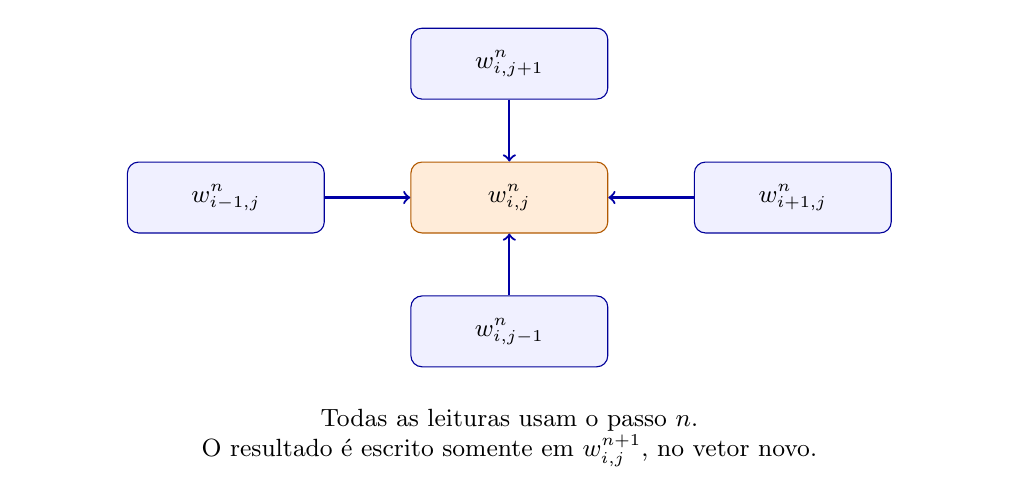
\begin{tikzpicture}[
    celula/.style={draw=blue!60!black,fill=blue!6,rounded corners,
                   minimum width=2.5cm,minimum height=.9cm,font=\small},
    dado/.style={->,thick,blue!65!black}]
\node[celula,fill=orange!15,draw=orange!70!black] (c) at (0,0) {$w^n_{i,j}$};
\node[celula] (l) at (-3.6,0) {$w^n_{i-1,j}$};
\node[celula] (r) at (3.6,0) {$w^n_{i+1,j}$};
\node[celula] (u) at (0,1.7) {$w^n_{i,j+1}$};
\node[celula] (d) at (0,-1.7) {$w^n_{i,j-1}$};
\draw[dado] (l)--(c);
\draw[dado] (r)--(c);
\draw[dado] (u)--(c);
\draw[dado] (d)--(c);
\node[align=center,font=\small,text width=12cm] at (0,-3.05)
{Todas as leituras usam o passo $n$.\\
O resultado é escrito somente em $w^{n+1}_{i,j}$, no vetor novo.};
\end{tikzpicture}
\caption{Estêncil de cinco pontos. A mesma atualização é aplicada separadamente a $u$ e $v$. A separação entre campos atuais e novos permite calcular células diferentes em paralelo.}
\label{fig:estencil}
\end{figure}
